\chapter{Pick and place points}
\label{pick_and_place}
This chapter explains the last steps in our algorithm, in which we use the data obtained in the previous garment analysis (chapter \ref{garment_analysis}) to determine the next unfold pick and place points for the humanoid robot.

\section{Candidate Unfold Paths}
\label{unfold_paths}

The next step in our algorithm is to create a set of paths from the highest point in the garment to the midpoint of each contour segment. This is the set of candidate unfold paths, based in the assumption that when a garment has an overlapping fold, the fold line will rest in the garment contour, and the folded surface with have lower depth values (i.e. closer to the depth sensor).

These paths are checked so that they are located entirely inside the garment, paths that go outside the garment contour are considered invalid. Figure \ref{fig:candidate_paths} shows both the initial path candidates set and the candidates set without the invalid paths.

\begin{figure}[thpb]
    \centering
    
\includegraphics[width=0.7
    \textwidth]{figures/placeholder2.png}
    \caption{\comment{(Figure that shows both the initial path candidate set and the candidate set without the invalid paths )}}
    \label{fig:candidate_paths}
\end{figure}


To find the highest point in the garment, regions found with the watershed algorithm are first averaged using the median value for each region. Then, the region with the lowest depth value, which is closer to the camera and therefore higher in the garment, is selected. The centroid of the selected cluster is the point selected as highest point. Using these method instead of selecting directly the highest point from the depth image increases the robustness of the algorithm against outliers and noise present in the depth image.



\section{Bumpiness}
\label{bumpiness}

\begin{equation}\label{bumpiness}
B = \sum_{i=1}^{n} | \textrm{path}(i)- \textrm{path}(i-1) | 
\end{equation}

Where $n$ is the number of points composing the path. The path with the lowest bumpiness value, which corresponds to the path with the less and smallest height changes, is selected as the unfold direction, Fig. \ref{fig:paths_with_bumpiness}.


\begin{figure}[thpb]
    \centering
    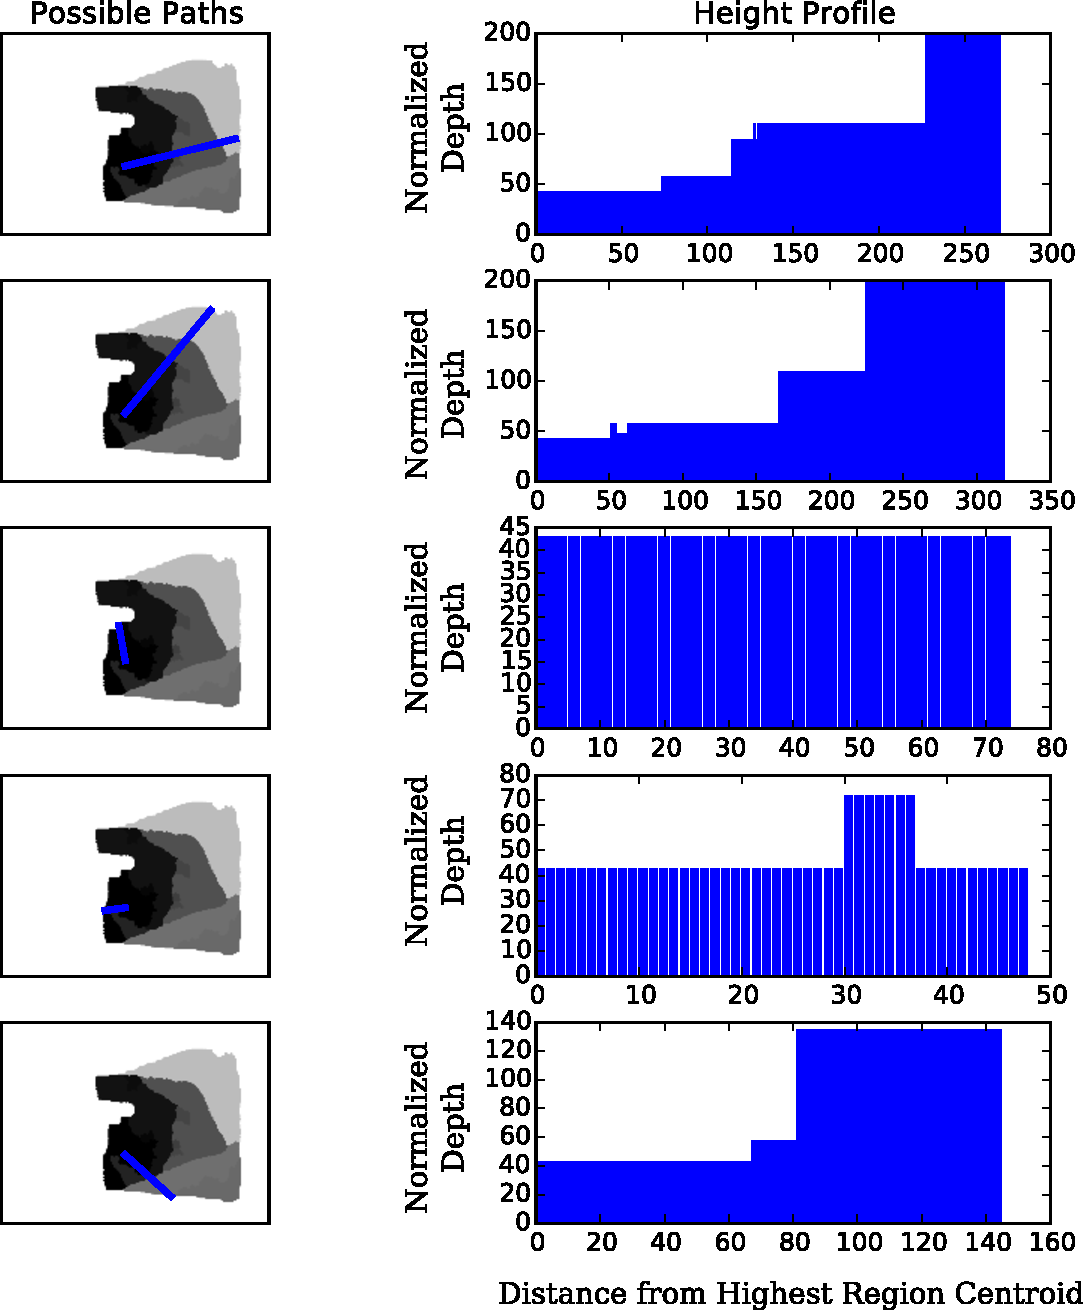
\includegraphics[width=0.48\textwidth]{figures/candidate_paths.pdf}
    \caption{On the left side, the candidate paths are shown. On the right side, the height profile of each path is shown. Notice that the depth sensor computes the distance to the object from itself, so that a low value in the bar plot means a closer object to the sensor, so it is a region with more height with respect to the table.}
    \label{fig:paths_with_bumpiness}
\end{figure}

\section{Pick and place points}
\label{pick_and_place}
\begin{figure}[thpb]
    \centering
    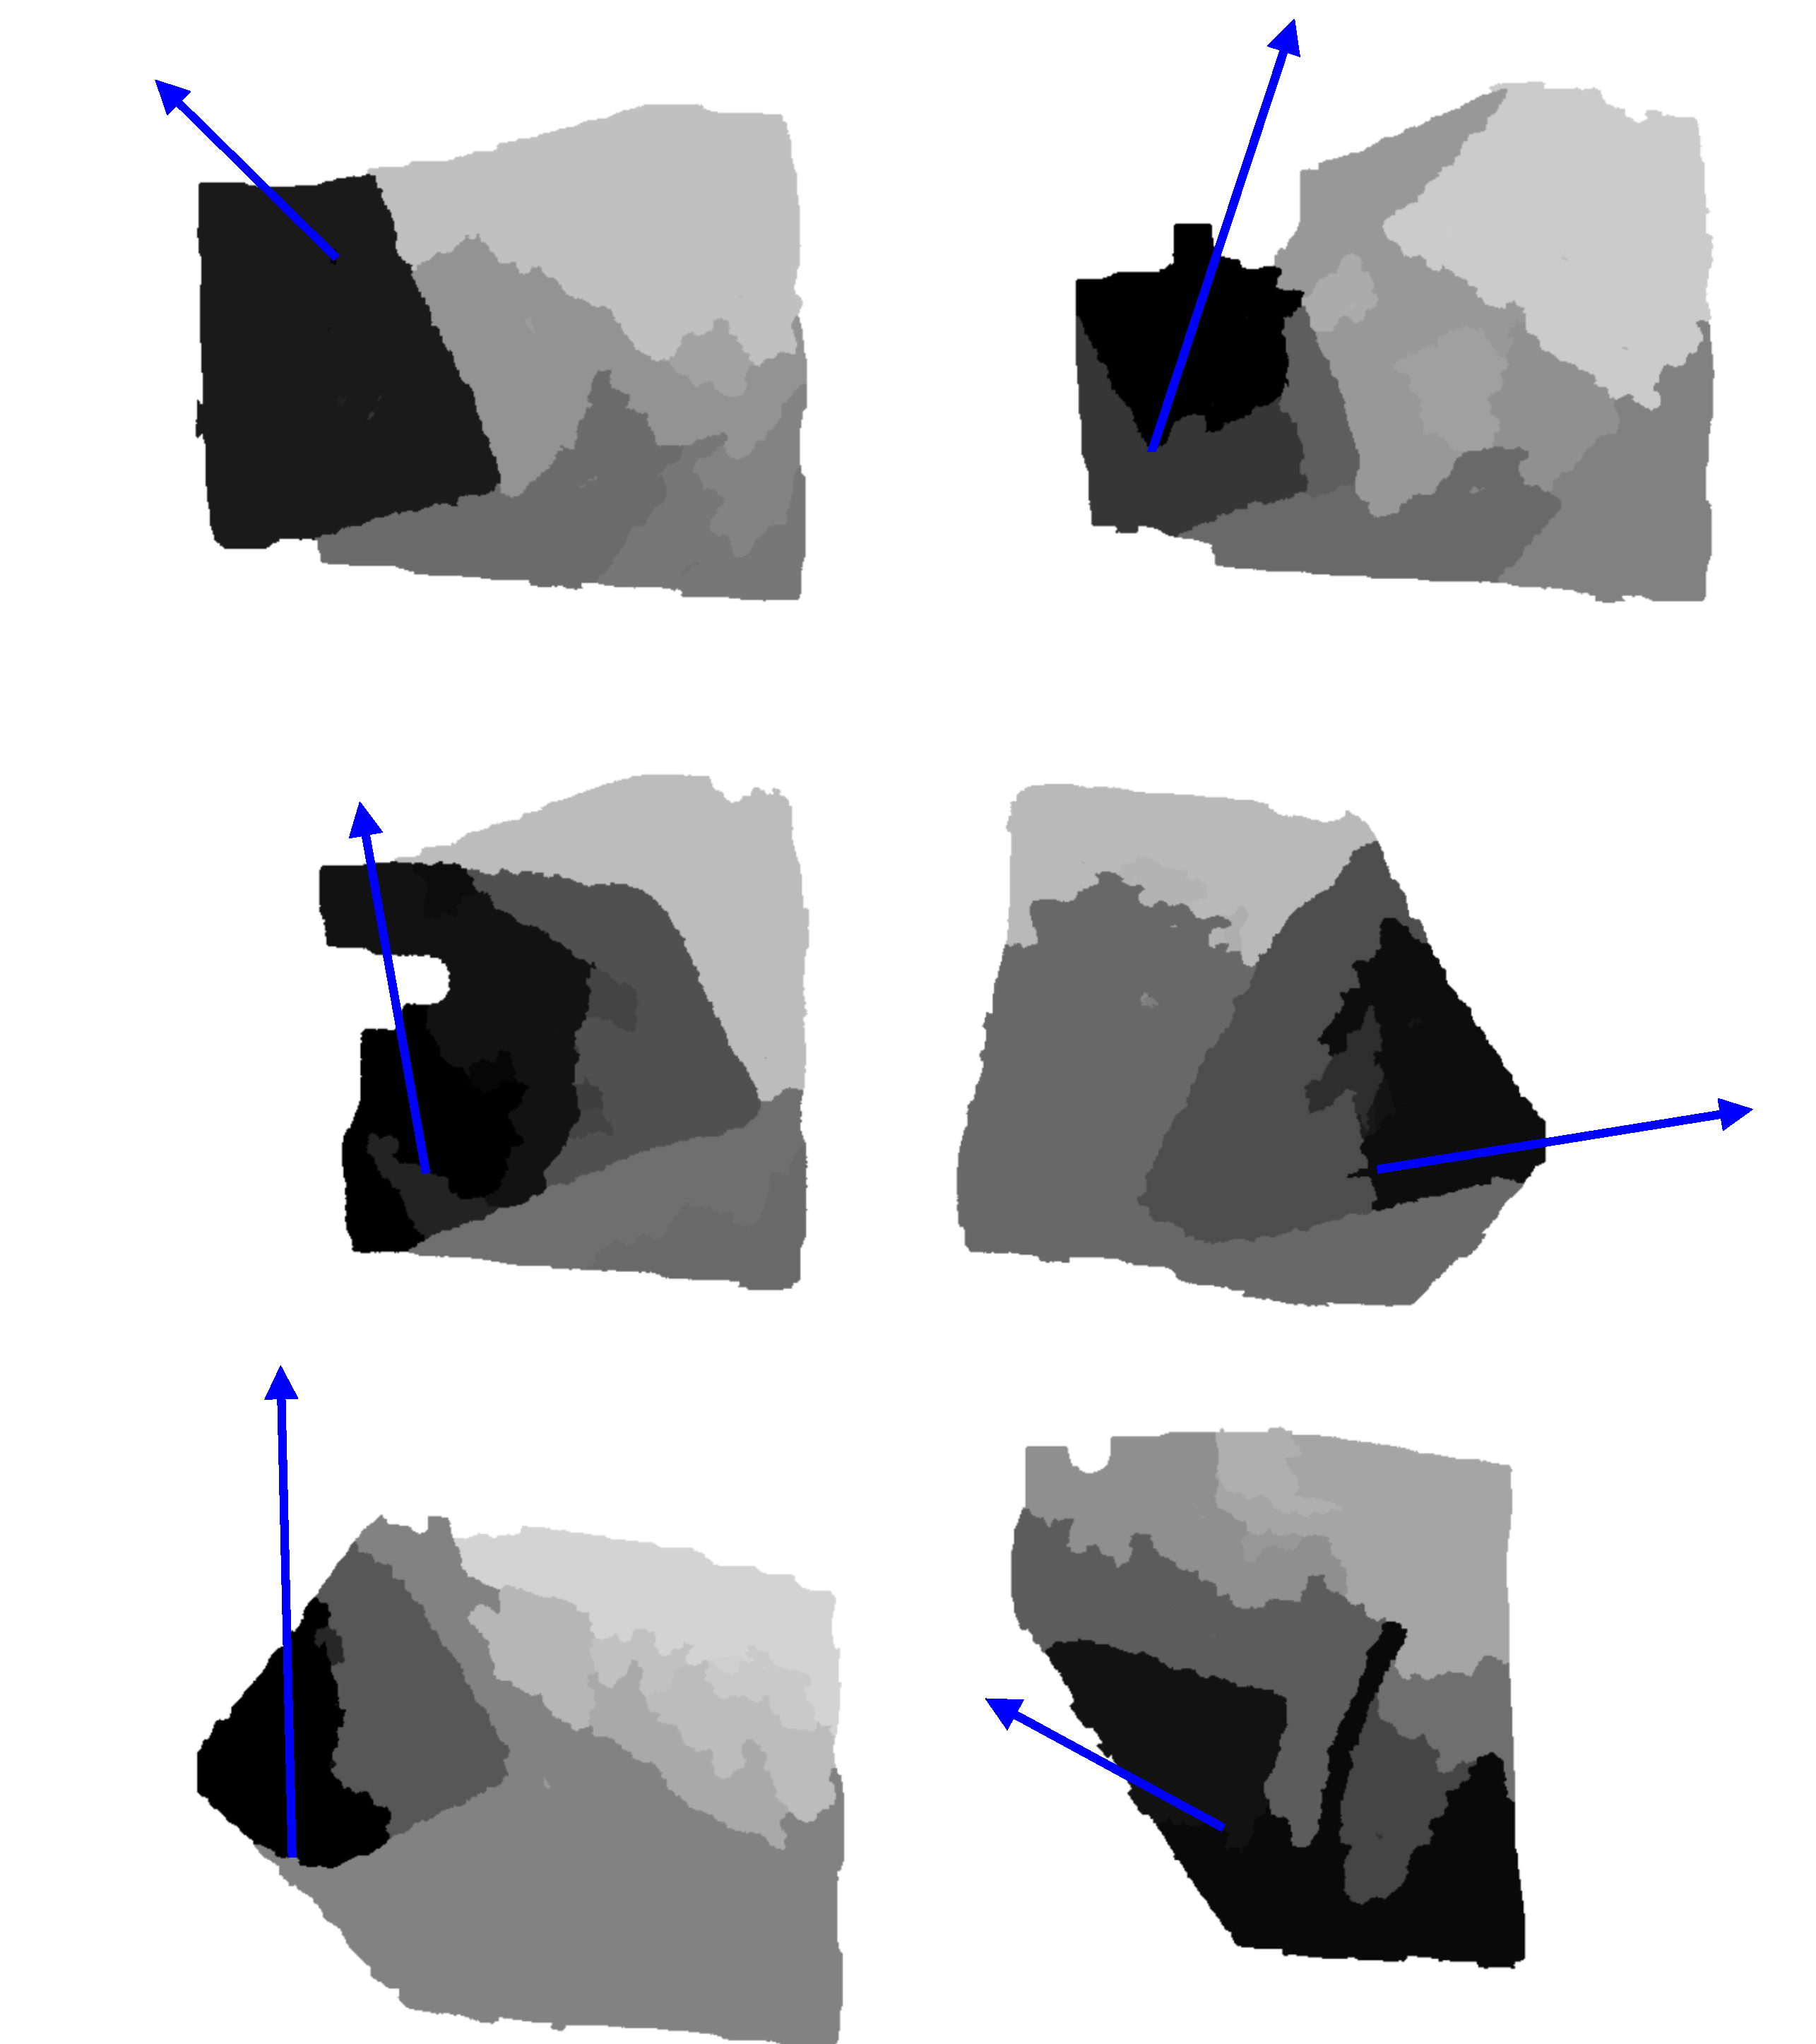
\includegraphics[width=0.45\textwidth]{figures/directions.pdf}
    \caption{Final directions calculated for each garment provided to the system. Each arrow departs where the robot should pick the fold and arrives where it should be placed.}
    \label{fig:directions}
\end{figure}